\chapter{Pilas, pilas de combustible y electrólisis}\label{ch:b2:batteries-electrolysis}

Cada kilogramo de aluminio obtenido de su mena cuesta unos \qty{13}{kW.h} de
electricidad; refundir un kilogramo de chatarra cuesta, en principio, los
\qty{0.3}{kW.h} que la calientan hasta su punto de fusión y la funden. La diferencia
es el trabajo de una larga hilera de cubas de \omterm{def:b2:batteries-electrolysis:electrolysis}{electrólisis}, cada una de las cuales hace pasar cientos de
miles de amperios a través de una sal fundida a unos pocos voltios. Una pila funciona en el
sentido contrario: una reacción espontánea impulsa la corriente. Con las
\omterm{def:b2:current-potential-curves:ie-curve}{curvas intensidad--potencial} del \cref{ch:b2:current-potential-curves}, ambas cosas se
leen en el mismo diagrama, y también un trozo de cinc que se disuelve en un ácido.
% ledger: hT:Al_l.933, aw:Al

\begin{recall}
\Cref{ch:b2:cell-thermodynamics}: $\Delta_r G = -nFE$, el trabajo máximo, la
\omterm{def:b2:cell-thermodynamics:faraday}{constante de Faraday}. \Cref{ch:b2:current-potential-curves}: \omterm{def:b2:current-potential-curves:ie-curve}{curvas
intensidad--potencial}, \omterm{def:b2:current-potential-curves:fast-slow}{sistemas rápidos} y lentos, \omterm{def:b2:current-potential-curves:overpotential}{sobretensiones}, \omterm{def:b2:current-potential-curves:limiting-current}{corrientes límite}, los muros del
agua. \Cref{ch:b2:ellingham}: por qué el aluminio no se obtiene con carbono. El volumen
escolar: \omterm{def:b2:batteries-electrolysis:electrolysis}{electrólisis}, \omterm{def:b2:batteries-electrolysis:battery}{acumuladores}.
\end{recall}

\begin{omfigure}
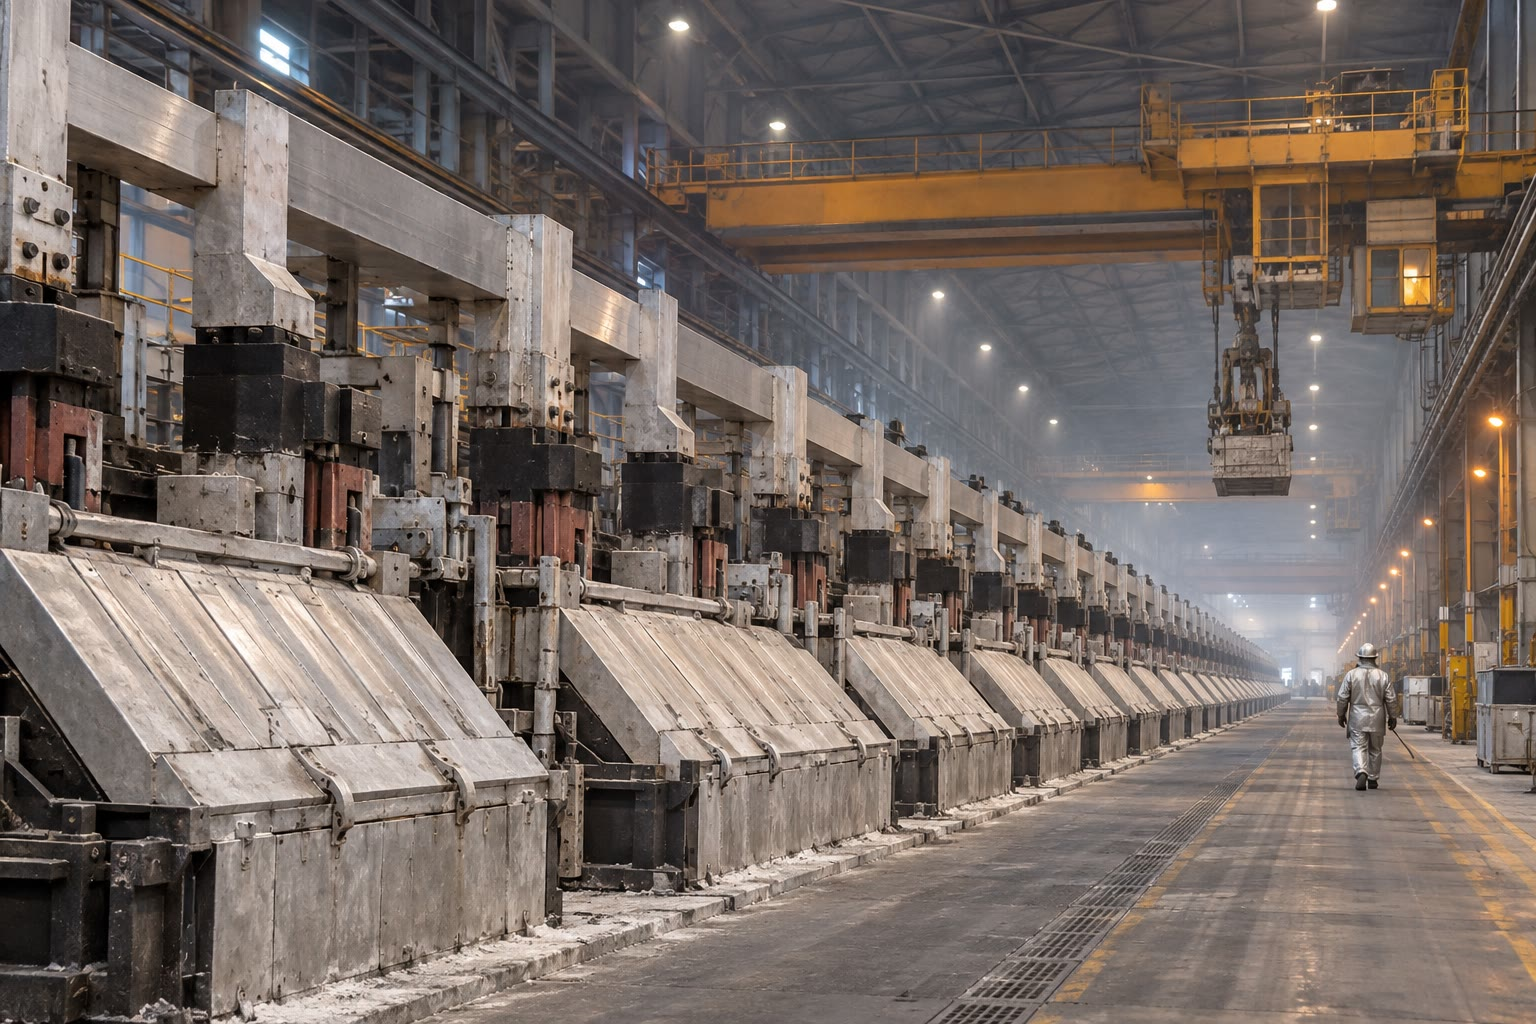
\includegraphics[width=0.62\linewidth]{images/book3/ai/b2-11-potroom.jpg}

{\small La nave de cubas de una fundición de aluminio: una hilera de cubas de \omterm{def:b2:batteries-electrolysis:electrolysis}{electrólisis},
de cientos de metros, conectadas en serie; la grúa puente cambia los ánodos de
carbono a medida que se consumen.}
\end{omfigure}

\section{Reacciones espontáneas leídas en las curvas}

\begin{definition}[Potencial mixto]\label{def:b2:batteries-electrolysis:mixed-potential}
El \emph{potencial mixto}\index{potencial mixto} de un electrodo sobre el que reaccionan dos
pares distintos, uno oxidándose y otro reduciéndose, es el potencial que
toma cuando no circula corriente neta: la \omterm{def:b2:current-potential-curves:ie-curve}{corriente anódica} de un par es entonces
igual y opuesta a la \omterm{def:b2:current-potential-curves:ie-curve}{corriente catódica} del otro.
\end{definition}

\begin{proposition}[Un metal en una disolución]\label{prop:b2:batteries-electrolysis:mixed}
Un metal sumergido en una disolución que puede oxidarlo se estabiliza en el potencial
$E_m$ en el que $i_a(E_m) = -i_c(E_m)$, compensando la \omterm{def:b2:current-potential-curves:ie-curve}{corriente anódica} de la oxidación del metal
la \omterm{def:b2:current-potential-curves:ie-curve}{corriente catódica} de la reducción del oxidante; el
metal se disuelve a la velocidad $i_a(E_m)/(nF)$.
\end{proposition}

\begin{proof}
Un trozo aislado de metal no transporta corriente neta. Ambas semirreacciones tienen lugar
en su superficie al mismo potencial, de modo que sus corrientes, leídas en sus curvas
a ese potencial, suman cero. Por la \cref{prop:b2:current-potential-curves:current-rate},
la \omterm{def:b2:current-potential-curves:ie-curve}{corriente anódica} da la velocidad de oxidación.
\end{proof}

\begin{omfigure}
\begin{tikzpicture}
\begin{axis}[omie, width=0.82\linewidth, height=6cm, xmin=-1.1, xmax=-0.3,
  ymin=-3, ymax=3, xlabel={$E$ (V)}, ylabel={$i$}, clip=true, clip mode=individual,
  axis y line=left]
\addplot[omanodic] table[x=E, y=i] {figdata/out/bachelor-2-ie-curves-f-Zn.dat};
\addplot[omcathodic] table[x=E, y=i] {figdata/out/bachelor-2-ie-curves-f-HZn.dat};
\addplot[omcathodic, dashed] table[x=E, y=i] {figdata/out/bachelor-2-ie-curves-f-HCu.dat};
\draw[densely dotted] (axis cs:-0.820,-0.148) -- (axis cs:-0.820,0.148);
\draw[densely dotted] (axis cs:-0.737,-2.38) -- (axis cs:-0.737,2.38);
\fill (axis cs:-0.820,0.148) circle (1.3pt); \fill (axis cs:-0.737,2.38) circle (1.3pt);
\node[font=\scriptsize, anchor=south east] at (axis cs:-0.825,0.2) {cinc solo};
\node[font=\scriptsize, anchor=west] at (axis cs:-0.73,2.38) {cinc en contacto con cobre};
\node[font=\scriptsize, omThm, anchor=west] at (axis cs:-0.70,1.2) {\ce{Zn} $\to$ \ce{Zn^2+}};
\node[font=\scriptsize, omDef, anchor=north west, align=left] at (axis cs:-0.87,-0.5) {\ce{H+} $\to$ \ce{H2}\\ sobre cinc};
\node[font=\scriptsize, omDef, anchor=north west] at (axis cs:-0.66,-1.7) {sobre cobre};
\end{axis}
\end{tikzpicture}

{\small Cinc en ácido (curvas modelo, iones cinc diluidos; potenciales de
$-1.1$ a \qty{-0.3}{V}). Solo, el cinc se estabiliza en
el \omterm{def:b2:batteries-electrolysis:mixed-potential}{potencial mixto} en el que su oxidación compensa la lenta reducción de
\ce{H+} sobre cinc: una corriente pequeña, una disolución lenta. En contacto con el cobre, sobre el que
la reducción de \ce{H+} es menos lenta, el equilibrio se desplaza a un potencial más alto
y a una corriente más de diez veces mayor: el cinc se disuelve deprisa, y el hidrógeno
burbujea sobre el cobre.}
\end{omfigure}

La misma lectura explica la corrosión (\cref{ch:b2:corrosion}): la velocidad de
corrosión de un metal es la corriente en su \omterm{def:b2:batteries-electrolysis:mixed-potential}{potencial mixto}.

\section{Pilas que suministran corriente}

\begin{definition}[Pilas y baterías]\label{def:b2:batteries-electrolysis:battery}
Una \emph{pila primaria}\index{pila primaria} es una pila electroquímica que se usa
una sola vez, hasta que se agotan sus reactivos. Un \emph{acumulador}\index{acumulador}
es una pila que puede recargarse haciendo pasar a la fuerza una corriente en el
sentido inverso, lo que invierte su reacción. La \emph{energía
específica}\index{energia especifica@energía específica} de una pila es la energía eléctrica que suministra
por unidad de masa, normalmente en \unit{W.h/kg}.
\end{definition}

\begin{proposition}[Tensión de una pila que suministra corriente]\label{prop:b2:batteries-electrolysis:delivering}
Una pila que suministra una corriente $I$ tiene una tensión
\[
  U = E_+ - E_- - \eta_a - |\eta_c| - rI ,
\]
donde $E_+$ y $E_-$ son los potenciales de equilibrio de sus dos electrodos,
$\eta_a > 0$ la \omterm{def:b2:current-potential-curves:overpotential}{sobretensión} de la oxidación en el electrodo negativo,
$\eta_c < 0$ la de la reducción en el electrodo positivo, y $r$ la
resistencia interna (electrolito, separador, conexiones).
\end{proposition}

\begin{proof}
La misma corriente $I$ es anódica en el electrodo negativo, cuyo potencial se
lee en su curva anódica, $E_- + \eta_a$, y catódica en el positivo,
cuyo potencial es $E_+ + \eta_c$. Entre ambos, la corriente atraviesa el
electrolito, donde el potencial cae en $rI$. Por tanto, $U = (E_+ + \eta_c) - (E_- +
\eta_a) - rI$.
\end{proof}

\begin{omfigure}
\begin{tikzpicture}
\begin{axis}[omie, width=0.82\linewidth, height=5.6cm, xmin=-1.2, xmax=0.8,
  ymin=-2, ymax=2, xlabel={$E$ (V)}, ylabel={$i$}, clip=true, clip mode=individual]
\addplot[omanodic] table[x=E, y=i] {figdata/out/bachelor-2-ie-curves-h-neg.dat};
\addplot[omcathodic] table[x=E, y=i] {figdata/out/bachelor-2-ie-curves-h-pos.dat};
\draw[densely dashed, gray] (axis cs:-1.2,1) -- (axis cs:0.8,1);
\draw[densely dashed, gray] (axis cs:-1.2,-1) -- (axis cs:0.8,-1);
\node[font=\scriptsize, gray, anchor=south west] at (axis cs:-1.18,1) {$+I$};
\node[font=\scriptsize, gray, anchor=north west] at (axis cs:-1.18,-1) {$-I$};
\fill (axis cs:-0.730,1) circle (1.3pt); \fill (axis cs:0.210,-1) circle (1.3pt);
\draw[densely dotted] (axis cs:-0.85,0) -- (axis cs:-0.85,0.5);
\draw[densely dotted] (axis cs:0.45,0) -- (axis cs:0.45,-0.5);
\node[font=\scriptsize, anchor=south] at (axis cs:-0.85,0.5) {$E_-$};
\node[font=\scriptsize, anchor=north] at (axis cs:0.45,-0.5) {$E_+$};
\draw[<->, thick, omProp] (axis cs:-0.730,1.5) -- (axis cs:0.210,1.5) node[midway, above, font=\scriptsize] {$U + rI$};
\draw[densely dotted] (axis cs:-0.730,1) -- (axis cs:-0.730,1.5);
\draw[densely dotted] (axis cs:0.210,-1) -- (axis cs:0.210,1.5);
\node[font=\scriptsize, omThm, anchor=west] at (axis cs:-0.70,0.6) {electrodo negativo};
\node[font=\scriptsize, omDef, anchor=west] at (axis cs:0.30,-1.5) {electrodo positivo};
\end{axis}
\end{tikzpicture}

{\small El punto de funcionamiento de una pila (curvas modelo). A una corriente $I$ el
electrodo negativo se sitúa en su curva anódica y el electrodo positivo en su
curva catódica; la diferencia de los dos potenciales, menos la caída óhmica
$rI$, es la tensión suministrada. Disminuye a medida que $I$ crece.}
\end{omfigure}

\begin{method}[El punto de funcionamiento de una pila o de un electrolizador]\label{met:b2:batteries-electrolysis:operating-point}
\begin{enumerate}
  \item Trácense la curva anódica del electrodo que se oxida y la
        curva catódica del que se reduce.
  \item Para una corriente $I$, léase el potencial de cada electrodo en $+I$ en la
        curva anódica y en $-I$ en la catódica.
  \item La diferencia de los dos potenciales, corregida en $rI$ (restada para
        una pila, sumada para un \omterm{def:b2:batteries-electrolysis:electrolysis}{electrolizador}), es la tensión.
\end{enumerate}
\end{method}

\begin{example}[El acumulador de plomo]\label{ex:b2:batteries-electrolysis:lead}
En el electrodo negativo, \ce{Pb + SO4^2- -> PbSO4 + 2e-}; en el positivo,
\ce{PbO2 + 4H+ + SO4^2- + 2e- -> PbSO4 + 2H2O}. En total,
\[
  \ce{Pb + PbO2 + 4H+ + 2SO4^2- -> 2PbSO4 + 2H2O},
\]
$\Delta_r G^\circ = 2(-813.14) + 2(-237.13) - (-217.33) - 2(-744.53) =
\qty{-394.1}{kJ/mol}$, $E^\circ = 394\,100/(2 \times 96\,485) = \qty{2.04}{V}$.
Ambos electrodos se recubren de sulfato de plomo a medida que la pila se descarga; la carga
invierte la reacción. La reducción de \ce{H+} sobre plomo y la oxidación del
agua sobre el dióxido de plomo son lentas: por eso una pila de \qty{2}{V} puede cargarse
en agua, cuya ventana termodinámica solo tiene \qty{1.23}{V} de anchura.
% ledger: dfg:PbSO4_cr, dfg:H2O_l, dfg:PbO2_cr, dfg:SO42-_ao
\end{example}

\begin{omfigure}
\begin{tikzpicture}[font=\small, >={Stealth}]
  \draw[thick] (0,0) rectangle (6,3.2);
  \fill[omDef!10] (0.05,0.05) rectangle (5.95,2.7);
  \fill[black!45] (0.6,0.4) rectangle (1.1,2.9);
  \fill[brown!60!black] (4.9,0.4) rectangle (5.4,2.9);
  \draw[thick] (0.85,2.9) -- (0.85,3.9) node[pos=0.75, left] {$-$};
  \draw[thick] (5.15,2.9) -- (5.15,3.9) node[pos=0.75, right] {$+$};
  \draw[->, thick, omProp] (0.85,3.9) -- (0.85,4.3) -- (5.15,4.3) -- (5.15,3.95);
  \node[font=\scriptsize, omProp, anchor=south] at (3,4.3) {$\mathrm{e^-}$ en la descarga};
  \node[font=\scriptsize, align=center] at (0.85,-0.45) {\ce{Pb}\\ (\ce{PbSO4} en la descarga)};
  \node[font=\scriptsize, align=center] at (5.15,-0.45) {\ce{PbO2}\\ (\ce{PbSO4} en la descarga)};
  \node[font=\scriptsize, align=center] at (3.0,1.6) {disolución de \ce{H2SO4}\\ \ce{H+}, \ce{HSO4-}, \ce{SO4^2-}};
\end{tikzpicture}

{\small El \omterm{def:b2:batteries-electrolysis:battery}{acumulador} de plomo, esquema. En la descarga el plomo se oxida
y el dióxido de plomo se reduce, ambos a sulfato de plomo, y se consume el ácido: la
densidad de la disolución indica el estado de carga.}
\end{omfigure}

\begin{omfigure}
\begin{tikzpicture}[font=\small, >={Stealth}]
  \draw[thick] (0,0) rectangle (7,3);
  % graphite layers
  \foreach \y in {0.5,0.9,1.3,1.7,2.1,2.5} \draw[thick, black!70] (0.3,\y) -- (2.3,\y);
  \foreach \y in {0.7,1.1,1.5,1.9,2.3} \foreach \x in {0.6,1.3,2.0} \fill[omDef] (\x,\y) circle (0.07);
  % layered oxide
  \foreach \y in {0.5,0.9,1.3,1.7,2.1,2.5} \draw[thick, omThm] (4.7,\y) -- (6.7,\y);
  \foreach \y in {0.7,1.5,2.3} \foreach \x in {5.0,5.7,6.4} \fill[omDef] (\x,\y) circle (0.07);
  \draw[densely dashed] (3.5,0) -- (3.5,3);
  \node[font=\scriptsize, align=center] at (1.3,-0.45) {grafito (negativo)};
  \node[font=\scriptsize, align=center] at (5.7,-0.45) {óxido laminar (positivo)};
  \node[font=\scriptsize, anchor=south] at (3.5,3.0) {separador};
  \draw[->, thick, omThm] (2.5,2.1) -- (4.5,2.1) node[midway, above, font=\scriptsize, fill=white, inner sep=1pt] {\ce{Li+} en la descarga};
  \draw[<-, thick, omDef] (2.5,0.9) -- (4.5,0.9) node[midway, below, font=\scriptsize, fill=white, inner sep=1pt] {\ce{Li+} en la carga};
\end{tikzpicture}

{\small Una celda de ion litio, esquema. Los iones litio (puntos azules) se alojan entre las
capas del grafito en la celda cargada; en la descarga atraviesan el
electrolito para deslizarse entre las capas de un óxido metálico, mientras los electrones dan
la vuelta por el circuito exterior. Ningún electrodo se disuelve ni se deposita: los
iones van y vienen entre dos anfitriones.}
\end{omfigure}

\begin{history}[La pila de Volta]
\begin{minipage}[t]{0.27\linewidth}
\vspace{0pt}
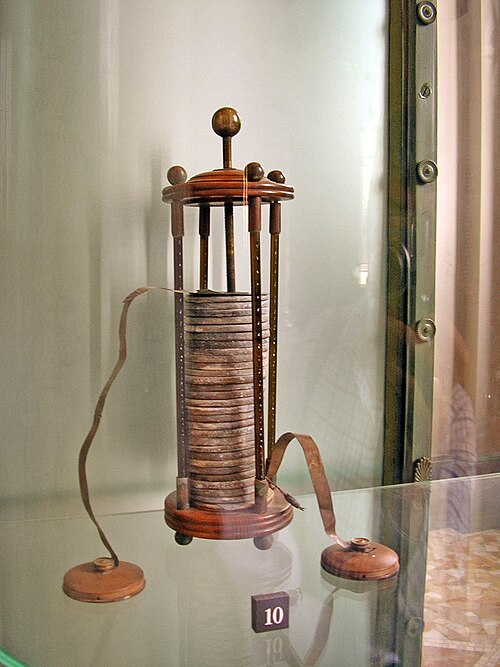
\includegraphics[width=\linewidth]{images/book3/volta-pile.jpg}
\end{minipage}\hfill
\begin{minipage}[t]{0.69\linewidth}
\vspace{0pt}
En 1800 Alessandro Volta describió una columna de discos de dos metales distintos,
cinc y cobre o plata, separados por tela empapada en salmuera: la primera
fuente de corriente eléctrica estable. En pocas semanas otros la usaron para descomponer
el agua, y en una década Humphry Davy había aislado el sodio y el potasio por
\omterm{def:b2:batteries-electrolysis:electrolysis}{electrólisis} de sus hidróxidos fundidos con una gran pila. La fotografía muestra
una de las pilas del propio Volta. (Fotografía: GuidoB, CC BY-SA 3.0, Wikimedia
Commons.)
\end{minipage}
\end{history}

\section{Pilas de combustible}

\begin{definition}[Pila de combustible]\label{def:b2:batteries-electrolysis:fuel-cell}
Una \emph{pila de combustible}\index{pila de combustible} es una pila cuyos reactivos, un combustible y un
oxidante (normalmente el oxígeno del aire), se alimentan de forma continua a sus
electrodos y cuyos productos se retiran, de modo que suministra corriente mientras
se la alimente.
\end{definition}

En la pila de membrana de intercambio de protones del autobús del
\cref{ch:b2:cell-thermodynamics}, el hidrógeno se oxida sobre un catalizador de platino,
\ce{H2 -> 2H+ + 2e-}, los protones atraviesan una fina membrana polimérica ácida, y el oxígeno se
reduce al otro lado, \ce{O2 + 4H+ + 4e- -> 2H2O}. La oxidación del hidrógeno
sobre platino es un \omterm{def:b2:current-potential-curves:fast-slow}{sistema rápido}; la reducción del oxígeno es lenta sobre cualquier
electrodo. La mayor parte de la tensión que se pierde entre los \qty{1.23}{V} de la pila
reversible y la tensión de trabajo es la \omterm{def:b2:current-potential-curves:overpotential}{sobretensión} del electrodo de oxígeno,
y el resto, la resistencia de la membrana y, a corriente alta, el aporte de
oxígeno al catalizador (una \omterm{def:b2:current-potential-curves:limiting-current}{corriente límite}).

\section{Electrólisis}

\begin{definition}[Electrólisis]\label{def:b2:batteries-electrolysis:electrolysis}
Una \emph{electrólisis}\index{electrolisis@electrólisis} es una reacción redox no espontánea
forzada por una corriente suministrada por un generador externo; la celda en la que
tiene lugar es un \emph{electrolizador}\index{electrolizador}. El ánodo, donde se
produce la oxidación, está conectado al polo positivo del generador.
\end{definition}

\begin{proposition}[Tensión mínima termodinámica]\label{prop:b2:batteries-electrolysis:minimum-voltage}
Una \omterm{def:b2:batteries-electrolysis:electrolysis}{electrólisis} cuya reacción tiene $\Delta_r G > 0$ requiere una tensión de al
menos $\Delta_r G/(nF)$.
\end{proposition}

\begin{proof}
El generador aporta el trabajo $nFU$ por mol de reacción; por el
\cref{thm:b2:cell-thermodynamics:delta-g-nfe} aplicado a la reacción inversa, el
trabajo eléctrico recibido debe ser al menos $\Delta_r G$.
\end{proof}

\begin{proposition}[Tensión de un electrolizador]\label{prop:b2:batteries-electrolysis:electrolysis-voltage}
Un \omterm{def:b2:batteries-electrolysis:electrolysis}{electrolizador} por el que pasa una corriente $I$ necesita
\[
  U = (E_a - E_c) + \eta_a + |\eta_c| + rI ,
\]
siendo $E_a$, $E_c$ los potenciales de equilibrio de los pares del ánodo y del cátodo
($E_a - E_c = \Delta_r G/(nF)$), $\eta_a$, $\eta_c$ sus \omterm{def:b2:current-potential-curves:overpotential}{sobretensiones} a esa
corriente y $r$ la resistencia entre los electrodos.
\end{proposition}

\begin{proof}
Como en una pila, la misma corriente es anódica en el ánodo, al potencial $E_a +
\eta_a$, y catódica en el cátodo, a $E_c + \eta_c$; el generador debe además
hacerla pasar por el electrolito, lo que añade $rI$.
\end{proof}

\begin{method}[Prever una electrólisis]\label{met:b2:batteries-electrolysis:predict-electrolysis}
\begin{enumerate}
  \item Enumérense todas las especies que pueden oxidarse en el ánodo (incluidos el
        metal del ánodo y el disolvente) y todas las que pueden reducirse en
        el cátodo (incluido el disolvente).
  \item Trácense sus \omterm{def:b2:current-potential-curves:ie-curve}{curvas intensidad--potencial} sobre los materiales de electrodo empleados.
  \item Al elevar la tensión, la primera curva anódica y la primera curva catódica
        alcanzadas dan las reacciones; a corrientes mayores, las siguientes añaden
        las suyas.
\end{enumerate}
\end{method}

\begin{definition}[Rendimiento faradaico]\label{def:b2:batteries-electrolysis:faradaic-efficiency}
El \emph{rendimiento faradaico}\index{rendimiento faradaico} $\eta_F$ de una
\omterm{def:b2:batteries-electrolysis:electrolysis}{electrólisis} es la fracción de la carga que ha pasado que produce el producto
deseado. Su \emph{consumo específico de energía}\index{consumo especifico de energia@consumo específico de energía}
es la energía eléctrica empleada por unidad de masa de producto.
\end{definition}

\begin{proposition}[Ley de Faraday]\label{prop:b2:batteries-electrolysis:faraday-mass}
Una corriente $I$ que pasa durante un tiempo $t$ con un \omterm{def:b2:batteries-electrolysis:faradaic-efficiency}{rendimiento faradaico} $\eta_F$ produce una
masa $m = \eta_F MIt/(nF)$ de un producto de masa molar $M$ formado con $n$
electrones por mol.
\end{proposition}

\begin{proof}
La carga $It$, de la cual $\eta_F It$ forma el producto, corresponde, por la
\cref{prop:b2:cell-thermodynamics:charge}, a $\eta_F It/(nF)$ moles.
\end{proof}

\begin{proposition}[Energía por kilogramo]\label{prop:b2:batteries-electrolysis:energy}
Con una tensión $U$ y un \omterm{def:b2:batteries-electrolysis:faradaic-efficiency}{rendimiento faradaico} $\eta_F$, el \omterm{def:b2:batteries-electrolysis:faradaic-efficiency}{consumo específico
de energía} es $w = nFU/(\eta_F M)$.
\end{proposition}

\begin{proof}
La energía es $UIt$ y la masa, $\eta_F MIt/(nF)$; se dividen.
\end{proof}

\section{Electrólisis industriales}

\paragraph{El cinc.} La mayor parte del cinc se obtiene por \omterm{def:b2:batteries-electrolysis:electrolysis}{electrólisis} de la disolución
ácida de sulfato de cinc del \cref{ch:b2:ellingham}. El cinc se deposita en el cátodo aunque
\ce{H+} sea el oxidante más fuerte: sobre cinc la reducción de \ce{H+} es muy lenta,
y la onda del cinc se alcanza primero; el ánodo desprende oxígeno.

\begin{omfigure}
\begin{tikzpicture}
\begin{axis}[omie, width=0.82\linewidth, height=5.6cm, xmin=-1.6, xmax=2.4,
  ymin=-2.4, ymax=2.4, xlabel={$E$ (V)}, ylabel={$i$}, clip=true, clip mode=individual]
\addplot[omcathodic] table[x=E, y=i] {figdata/out/bachelor-2-ie-curves-g-cath.dat};
\addplot[omanodic] table[x=E, y=i] {figdata/out/bachelor-2-ie-curves-g-an.dat};
\draw[densely dotted] (axis cs:-0.76,-2.2) -- (axis cs:-0.76,0.4);
\draw[densely dotted] (axis cs:0,-2.2) -- (axis cs:0,0.4);
\node[font=\scriptsize, anchor=south] at (axis cs:-0.76,0.4) {$-0.76$};
\node[font=\scriptsize, anchor=south east] at (axis cs:-0.02,0.4) {$0$};
\node[font=\scriptsize, omDef, anchor=north west, align=left] at (axis cs:-0.7,-1.05) {\ce{Zn^2+} $\to$ \ce{Zn},\\ meseta};
\node[font=\scriptsize, omDef, anchor=east, align=right] at (axis cs:-1.32,-0.9) {\ce{H+} $\to$ \ce{H2}\\ sobre Zn};
\node[font=\scriptsize, omThm, anchor=east] at (axis cs:1.85,1.6) {\ce{H2O} $\to$ \ce{O2}};
\node[font=\scriptsize, gray, align=center] at (axis cs:-0.38,-0.5) {aquí no hay \ce{H2}\\ sobre cinc};
\end{axis}
\end{tikzpicture}

{\small \omterm{def:b2:batteries-electrolysis:electrolysis}{Electrólisis} de una disolución ácida de sulfato de cinc con un cátodo de cinc
(curvas modelo). Aunque el par \ce{H+}/\ce{H2} ($\qty{0}{V}$) está por encima de
\ce{Zn^2+}/\ce{Zn} ($\qty{-0.76}{V}$), la reducción de \ce{H+} sobre cinc no
empieza antes de unos \qty{-1.1}{V}: entre ambos, el cinc se deposita solo. En el
ánodo, el agua se oxida a oxígeno.}
\end{omfigure}

\paragraph{El cloro y el hidróxido de sodio.} La salmuera se electroliza en una celda
dividida por una membrana que solo deja pasar los cationes. En el ánodo el cloruro se
oxida, \ce{2Cl- -> Cl2 + 2e-}; en el cátodo se reduce el agua, \ce{2H2O +
2e- -> H2 + 2OH-}; los iones sodio atraviesan la membrana para compensar la carga, y una
disolución de hidróxido de sodio sale del lado del cátodo, libre de cloruro. El
mínimo termodinámico es $\Delta_r G/(2F) = \qty{2.19}{V}$ para \ce{2Cl- + 2H2O -> Cl2 +
H2 + 2OH-} en condiciones estándar. En el ánodo se forma cloro y no
oxígeno, aunque el par \ce{O2}/\ce{H2O} esté más abajo: la oxidación del agua
es la más lenta de las dos sobre los materiales de ánodo empleados.
% ledger: dfg:OH-_ao, dfg:Cl-_ao, dfg:H2O_l

\begin{omfigure}
\begin{tikzpicture}[font=\small, >={Stealth}]
  \draw[thick] (0,0) rectangle (6,3.4);
  \draw[thick, dashed, omProp] (3,0) -- (3,3.4);
  \fill[black!30] (0.4,0.3) rectangle (0.7,3.0);
  \fill[black!50] (5.3,0.3) rectangle (5.6,3.0);
  \node[font=\scriptsize] at (0.55,3.3) {$+$};
  \node[font=\scriptsize] at (5.45,3.3) {$-$};
  \node[font=\scriptsize, align=center] at (1.85,1.9) {salmuera\\ \ce{2Cl-} $\to$\\ \ce{Cl2 + 2e-}};
  \node[font=\scriptsize, align=center] at (4.2,1.9) {disolución\\ de \ce{NaOH}\\ \ce{2H2O + 2e-} $\to$\\ \ce{H2 + 2OH-}};
  \draw[->, thick, omDef] (2.6,0.8) -- (3.4,0.8) node[pos=0.1, above, font=\scriptsize] {\ce{Na+}};
  \draw[->, thick] (1.0,3.4) -- (1.0,4.0) node[above] {\ce{Cl2}};
  \draw[->, thick] (5.0,3.4) -- (5.0,4.0) node[above] {\ce{H2}};
  \draw[->, thick] (-0.8,0.6) -- (0,0.6) node[pos=0, left] {entrada de salmuera};
  \draw[->, thick] (6,0.6) -- (6.8,0.6) node[right] {salida de \ce{NaOH}};
  \node[font=\scriptsize, omProp, anchor=north] at (3,-0.05) {membrana de intercambio catiónico};
\end{tikzpicture}

{\small Una celda cloro-álcali de membrana, esquema. Solo los iones sodio atraviesan la
membrana, de modo que el hidróxido formado en el cátodo no se encuentra con el cloro.}
\end{omfigure}

\paragraph{El aluminio.} El óxido de aluminio se disuelve en criolita fundida,
\ce{Na3AlF6}, que funde a una temperatura mucho más baja que la alúmina, y se electroliza entre un
cátodo de carbono, sobre el que se acumula el aluminio líquido, y ánodos de carbono que
se consumen en forma de dióxido de carbono (proceso Hall--Héroult):
\[
  \ce{2Al2O3 + 3C -> 4Al + 3CO2} .
\]
El mínimo termodinámico hacia \qty{1250}{K} es de unos \qty{1.18}{V}
(\cref{pb:b2:batteries-electrolysis:1}); la cuba de ese problema trabaja a tres
veces y media ese valor, y el exceso se convierte en el calor que mantiene fundido el
baño.

\begin{omfigure}
\begin{tikzpicture}[font=\small, >={Stealth}]
  \draw[thick, fill=black!12] (0,0) rectangle (7,3.2);
  \fill[black!45] (0.3,0.3) rectangle (6.7,0.8);
  \fill[gray!35] (0.3,0.8) rectangle (6.7,1.4);
  \fill[orange!30] (0.3,1.4) rectangle (6.7,2.5);
  \foreach \x in {1.0,3.0,5.0} {
    \fill[black!75] (\x,1.75) rectangle (\x+1.0,3.6);
    \draw[thick] (\x+0.5,3.6) -- (\x+0.5,4.2);
  }
  \draw[thick] (1.5,4.2) -- (5.5,4.2) node[right] {$+$};
  \node[font=\scriptsize, align=left, anchor=west] at (7.3,2.6) {ánodos de carbono, quemados a \ce{CO2}};
  \node[font=\scriptsize, align=left, anchor=west] at (7.3,1.95) {criolita fundida + \ce{Al2O3} disuelta};
  \node[font=\scriptsize, align=left, anchor=west] at (7.3,1.1) {aluminio líquido (cátodo)};
  \node[font=\scriptsize, align=left, anchor=west] at (7.3,0.55) {bloque catódico de carbono, $-$};
  \draw[densely dotted] (6.7,2.6) -- (7.3,2.6) (6.7,1.95) -- (7.3,1.95) (6.7,1.1) -- (7.3,1.1) (6.7,0.55) -- (7.3,0.55);
\end{tikzpicture}

{\small Una cuba Hall--Héroult, corte transversal, esquema. El aluminio se reduce
en la superficie del charco de metal líquido, que actúa como cátodo; los iones óxido
se descargan sobre los ánodos de carbono, que queman a dióxido de carbono.}
\end{omfigure}

\begin{history}[Hall y Héroult, 1886]
\begin{minipage}[t]{0.18\linewidth}
\vspace{0pt}
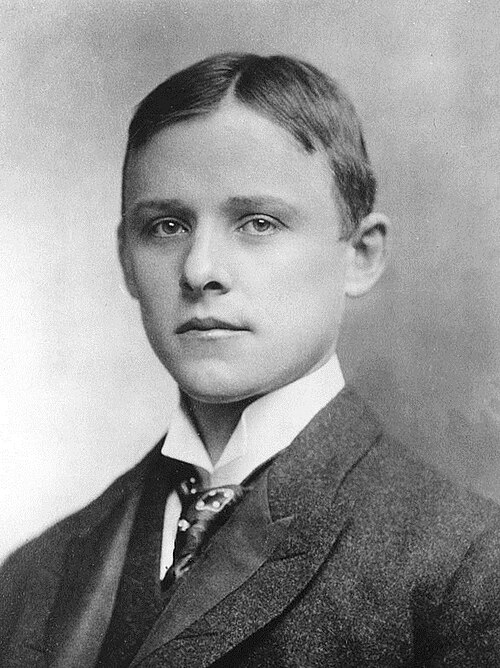
\includegraphics[width=\linewidth]{images/book3/hall.jpg}
\end{minipage}\hspace{0.02\linewidth}%
\begin{minipage}[t]{0.18\linewidth}
\vspace{0pt}
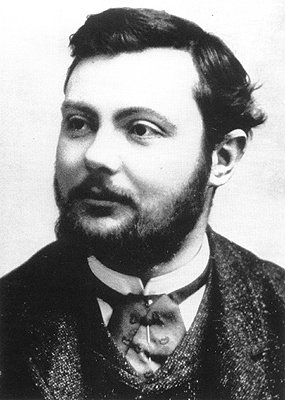
\includegraphics[width=\linewidth]{images/book3/heroult.jpg}
\end{minipage}\hfill
\begin{minipage}[t]{0.58\linewidth}
\vspace{0pt}
En 1886, con veintidós o veintitrés años, Charles Martin Hall y
Paul Héroult, a ambos lados del Atlántico, descubrieron de forma independiente que la alúmina
se disuelve en criolita fundida y puede electrolizarse en ella. El aluminio, hasta
entonces un metal precioso que se obtenía reduciendo su cloruro con sodio, se convirtió en el
más barato de los metales ligeros en cuanto pudo generarse electricidad a gran escala.
(Retratos: Hall, hacia la década de 1880, autor desconocido, dominio público; Héroult,
dominio público; Wikimedia Commons.)
\end{minipage}
\end{history}

\paragraph{El sodio.} El sodio no puede depositarse a partir del agua, que reduce.
Se obtiene por \omterm{def:b2:batteries-electrolysis:electrolysis}{electrólisis} del cloruro de sodio fundido, cuyo punto de fusión
se rebaja con una sal añadida (una \omterm{def:b2:solid-liquid-diagrams:eutectic}{mezcla eutéctica}, \cref{ch:b2:solid-liquid-diagrams}),
con cloro como subproducto. A \qty{1100}{K}, $\Delta_f G^\circ(\ce{NaCl}, \text{l}) =
\qty{-310.7}{kJ/mol}$: la tensión mínima es de \qty{3.22}{V}.
% ledger: janafG:NaCl.1100

\section{Ejercicios}

\begin{exercise}[$\star$]\label{exo:b2:batteries-electrolysis:1}
En la figura del cinc en ácido, léanse el \omterm{def:b2:batteries-electrolysis:mixed-potential}{potencial mixto} y la corriente del cinc
solo y del cinc en contacto con cobre (unidades del modelo), y dígase cuál se disuelve
más deprisa.
\end{exercise}

\begin{exercise}[$\star$]\label{exo:b2:batteries-electrolysis:2}
¿Qué masa de cinc se deposita en una hora con una corriente de \qty{500}{A} y un
\omterm{def:b2:batteries-electrolysis:faradaic-efficiency}{rendimiento faradaico} del 100~\%?
\end{exercise}

\begin{exercise}[$\star$]\label{exo:b2:batteries-electrolysis:3}
Calcúlese la tensión estándar del \omterm{def:b2:batteries-electrolysis:battery}{acumulador} de plomo a partir de las \omterm{def:b2:reaction-free-energy:gibbs-energy}{energías de Gibbs}
de formación dadas en el capítulo, y el número de celdas de una batería de coche de
\qty{12}{V}.
\end{exercise}

\begin{exercise}[$\star$]\label{exo:b2:batteries-electrolysis:4}
¿Qué carga, en amperios hora, puede suministrar un gramo de litio si se oxida
por completo a \ce{Li+}?
\end{exercise}

\begin{exercise}[$\star\star$]\label{exo:b2:batteries-electrolysis:5}
Una celda de afino de cobre hace pasar \qty{200}{A} durante \qty{24}{h} y deposita
\qty{5.50}{kg} de cobre. Calcúlese el \omterm{def:b2:batteries-electrolysis:faradaic-efficiency}{rendimiento faradaico}.
\end{exercise}

\begin{exercise}[$\star\star$]\label{exo:b2:batteries-electrolysis:6}
Una cuba de electroobtención de cinc trabaja a \qty{3.3}{V} con un \omterm{def:b2:batteries-electrolysis:faradaic-efficiency}{rendimiento faradaico} del
90~\% (datos del ejercicio). Calcúlese la energía eléctrica por kilogramo de cinc.
\end{exercise}

\begin{exercise}[$\star\star$]\label{exo:b2:batteries-electrolysis:7}
Una pila da \qty{1.55}{V} a \qty{0.10}{A} y \qty{1.40}{V} a \qty{0.60}{A}.
Suponiendo despreciables las \omterm{def:b2:current-potential-curves:overpotential}{sobretensiones}, hállense su resistencia interna y su
tensión sin corriente.
\end{exercise}

\begin{exercise}[$\star\star$]\label{exo:b2:batteries-electrolysis:8}
Se electroliza salmuera en la celda de membrana. Escríbanse las reacciones de electrodo,
calcúlese la tensión mínima y explíquese por qué los productos deben mantenerse
separados.
\end{exercise}

\begin{exercise}[$\star\star$]\label{exo:b2:batteries-electrolysis:9}
Calcúlense la tensión mínima para la \omterm{def:b2:batteries-electrolysis:electrolysis}{electrólisis} del cloruro de sodio fundido a
\qty{1100}{K} y la energía mínima por kilogramo de sodio.
\end{exercise}

\begin{exercise}[$\star\star\star$]\label{exo:b2:batteries-electrolysis:10}
Con \omterm{def:b2:current-potential-curves:ie-curve}{curvas intensidad--potencial}, explíquese por qué puede depositarse cinc a partir de un baño ácido
sobre un cátodo de cinc, y predígase qué ocurriría sobre un cátodo de platino al
principio del depósito.
\end{exercise}

\begin{exercise}[$\star\star\star$]\label{exo:b2:batteries-electrolysis:11}
A partir de $\Delta_f G^\circ$ a \qty{1100}{K} y \qty{1300}{K} ($\ce{Al2O3}$: $-1328.3$ y
$-1262.3$; $\ce{CO2}$: $-396.0$ y $-396.2$ \unit{kJ/mol}), calcúlese la tensión
mínima de la cuba Hall--Héroult a \qty{1250}{K}, y compárese con un
ánodo inerte en el que se desprendería oxígeno.
\end{exercise}

\begin{exercise}[$\star\star\star$]\label{exo:b2:batteries-electrolysis:12}
Se almacena electricidad electrolizando agua a \qty{1.80}{V} y se recupera en una
\omterm{def:b2:batteries-electrolysis:fuel-cell}{pila de combustible} a \qty{0.70}{V}, ambas con un \omterm{def:b2:batteries-electrolysis:faradaic-efficiency}{rendimiento faradaico} del 100~\%. Calcúlese el
rendimiento del ciclo completo y explíquese adónde va la energía.
\end{exercise}

\section{Problema: una tonelada de aluminio}

\begin{problem}[{Problema de fin de semana --- la reacción de la cuba Hall--Héroult
y su tensión mínima, la carga y el tiempo para producir una tonelada de aluminio,
la energía empleada y el carbono quemado}]
\label{pb:b2:batteries-electrolysis:1}
Datos: \omterm{def:b2:reaction-free-energy:gibbs-energy}{energías de Gibbs} de formación JANAF a \qty{1100}{K} y \qty{1300}{K}
(\unit{kJ/mol}): \ce{Al2O3} $-1328.3$, $-1262.3$; \ce{CO2} $-396.0$, $-396.2$. Cuba
(datos del ejercicio): corriente \qty{300}{kA}, tensión \qty{4.1}{V}, \omterm{def:b2:batteries-electrolysis:faradaic-efficiency}{rendimiento faradaico}
94~\%, baño hacia \qty{1250}{K}. Masas molares (\unit{g/mol}): Al 26.982, C 12.011,
O 15.999. Calor necesario para llevar el aluminio de \qty{298}{K} al estado líquido en su punto de
fusión: \qty{28.69}{kJ/mol}.
% ledger: janafG:Al2O3.1100, janafG:Al2O3.1300, janafG:CO2.1100, janafG:CO2.1300, aw:Al, aw:C, aw:O, hT:Al_l.933, const:F

\medskip
\noindent\textbf{Parte I --- La tensión mínima.}
\begin{enumerate}
  \item Dense los números de oxidación del aluminio, el oxígeno y el carbono en los
        reactivos y en los productos.
  \item Escríbanse las semirreacciones del cátodo y del ánodo, con el ion óxido
        \ce{O^2-} transportado por el baño fundido.
  \item Escríbanse la reacción global y el número $n$ de electrones intercambiados.
  \item Interpólense los $\Delta_f G^\circ$ de \ce{Al2O3} y \ce{CO2} a \qty{1250}{K}.
  \item Calcúlese $\Delta_r G^\circ$ a \qty{1250}{K}.
  \item Dedúzcase la tensión mínima.
  \item Calcúlese la tensión mínima con un ánodo inerte,
        \ce{2Al2O3 -> 4Al + 3O2}, y explíquese el papel del carbono.
\end{enumerate}

\medskip
\noindent\textbf{Parte II --- Carga y tiempo.}
\begin{enumerate}[resume]
  \item ¿Qué cantidad de aluminio hay en una tonelada?
  \item ¿Qué carga haría falta con un \omterm{def:b2:batteries-electrolysis:faradaic-efficiency}{rendimiento faradaico} del 100~\%?
  \item ¿Qué carga se hace pasar en realidad?
  \item ¿Cuánto tarda una cuba en producir una tonelada?
  \item ¿Qué masa de aluminio produce una cuba al día?
  \item Propóngase adónde va el 6~\% de carga perdido.
\end{enumerate}

\medskip
\noindent\textbf{Parte III --- Energía.}
\begin{enumerate}[resume]
  \item Calcúlese la energía eléctrica por tonelada.
  \item Exprésese en \unit{kW.h} por kilogramo.
  \item Calcúlese la energía mínima por kilogramo, a la tensión mínima y con un
        rendimiento del 100~\%.
  \item ¿Adónde va el resto de la energía, y por qué no se desperdicia
        del todo?
  \item Calcúlese la potencia eléctrica de una cuba.
  \item Calcúlese el calor necesario para refundir un kilogramo de chatarra, en
        \unit{kW.h}, y compárese.
  \item ¿Qué fracción de la tensión de trabajo representa el mínimo termodinámico?
\end{enumerate}

\medskip
\noindent\textbf{Parte IV --- El carbono.}
\begin{enumerate}[resume]
  \item Calcúlese la masa de carbono quemada por tonelada de aluminio según la
        ecuación.
  \item Calcúlese la masa de dióxido de carbono liberada por los ánodos por tonelada.
  \item Las cubas reales queman más carbono que eso. Propónganse dos razones.
  \item Exprésese el \ce{CO2} anódico por kilogramo de aluminio.
  \item ¿Qué cambiaría un ánodo inerte en la tensión y en el gas
        liberado?
  \item Indíquese la energía eléctrica por kilogramo de aluminio.
\end{enumerate}
\end{problem}
